%\section*{\lbtitle Наблюдение плазмолиза}
%\addcontentsline{toc}{section}{Наблюдение плазмолиза}

%\subsection*{Теоретические положения}

%\paragraph{}Роль цитоплазматической мембраны в обмене веществ клетки заключается в контроле транспорта веществ между клеткой и окружающей средой. За счёт избирательной проницаемости, цитоплазматическая мембрана обеспечивает постоянство внутренней среды клетки и поддерживает состояния \hyperlink{gomiostatsis_question}{гомеостаза} с окружающей средой. Утрата клеточной мембраной избирательной проницаемости приводит к гибели клетки, так как мембрана теряет способность удерживать внутри клетки воду и необходимые минеральные элементы. 

%\paragraph{}Потеря клеткой воды сопровождается плазмолизом.

%\paragraph{}Мезоплазма – слои цитоплазмы между плазмолеммой и тонопластом, включает органеллы и гиалоплазму. Важным ее свойством является структурная вязкость, обеспечиваемая взаимодействием молекул воды с коллоидами и ионами. Вязкость цитоплазмы влияет на ход и направленность действия ферментов. В качестве регуляторов вязкости выступают ионы K+ и Ca2+. Калий снижает вязкость, а кальций ее увеличивает. Поддержание определенной вязкости достигается определенным соотношением одно- и двухвалентных катионов. Для изучения влияния ионов на вязкость цитоплазмы можно использовать наблюдение плазмолиза.

%\paragraph{}\efbox[margin=10pt,backgroundcolor=yellow]{
%	\begin{minipage}{0.95\textwidth}
%	\textbf{Плазмолиз} это процесс отставания цитоплазмы от стенок клетки, помещённой в раствор, концентрация солей в котором превышает концентрацию клеточного сока (гипертонический раствор)
%	\end{minipage}
%	} 

%\paragraph{}Под микроскопом можно наблюдать, как в ходе плазмолиза форма протопласта начинает меняться. Вначале протопласт отстает от клеточной стенки только в отдельных местах, чаще всего в уголках клетки. Плазмолиз такой формы называют \textit{уголковым} (рисунок \ref{plasmolis_types}: 1). Постепенно протопласт настолько сильно отделяется от клеточной стенки, что связь с ней сохраняется лишь в отдельных её участках. При этом, поверхность протопласта между этими участками имеет вогнутую форму. На этом этапе плазмолиз называется \textit{вогнутым}. В конце концов, протопласт полностью отрывается от клеточных стенок и принимает округлую форму. Такой плазмолиз носит название \textit{выпуклый}.

%%%%%%%%%%%%%%%%%%%%%%%%%%%%%%%%%%%%%%%%%%%%%%%%%%%%%%%%%%%%%%%%%%%%%%%%%%%%%%%%%%%%%%%%%%%%%%%%%%%%%%%%%%% 
%\begin{figure}
%  \centering
%       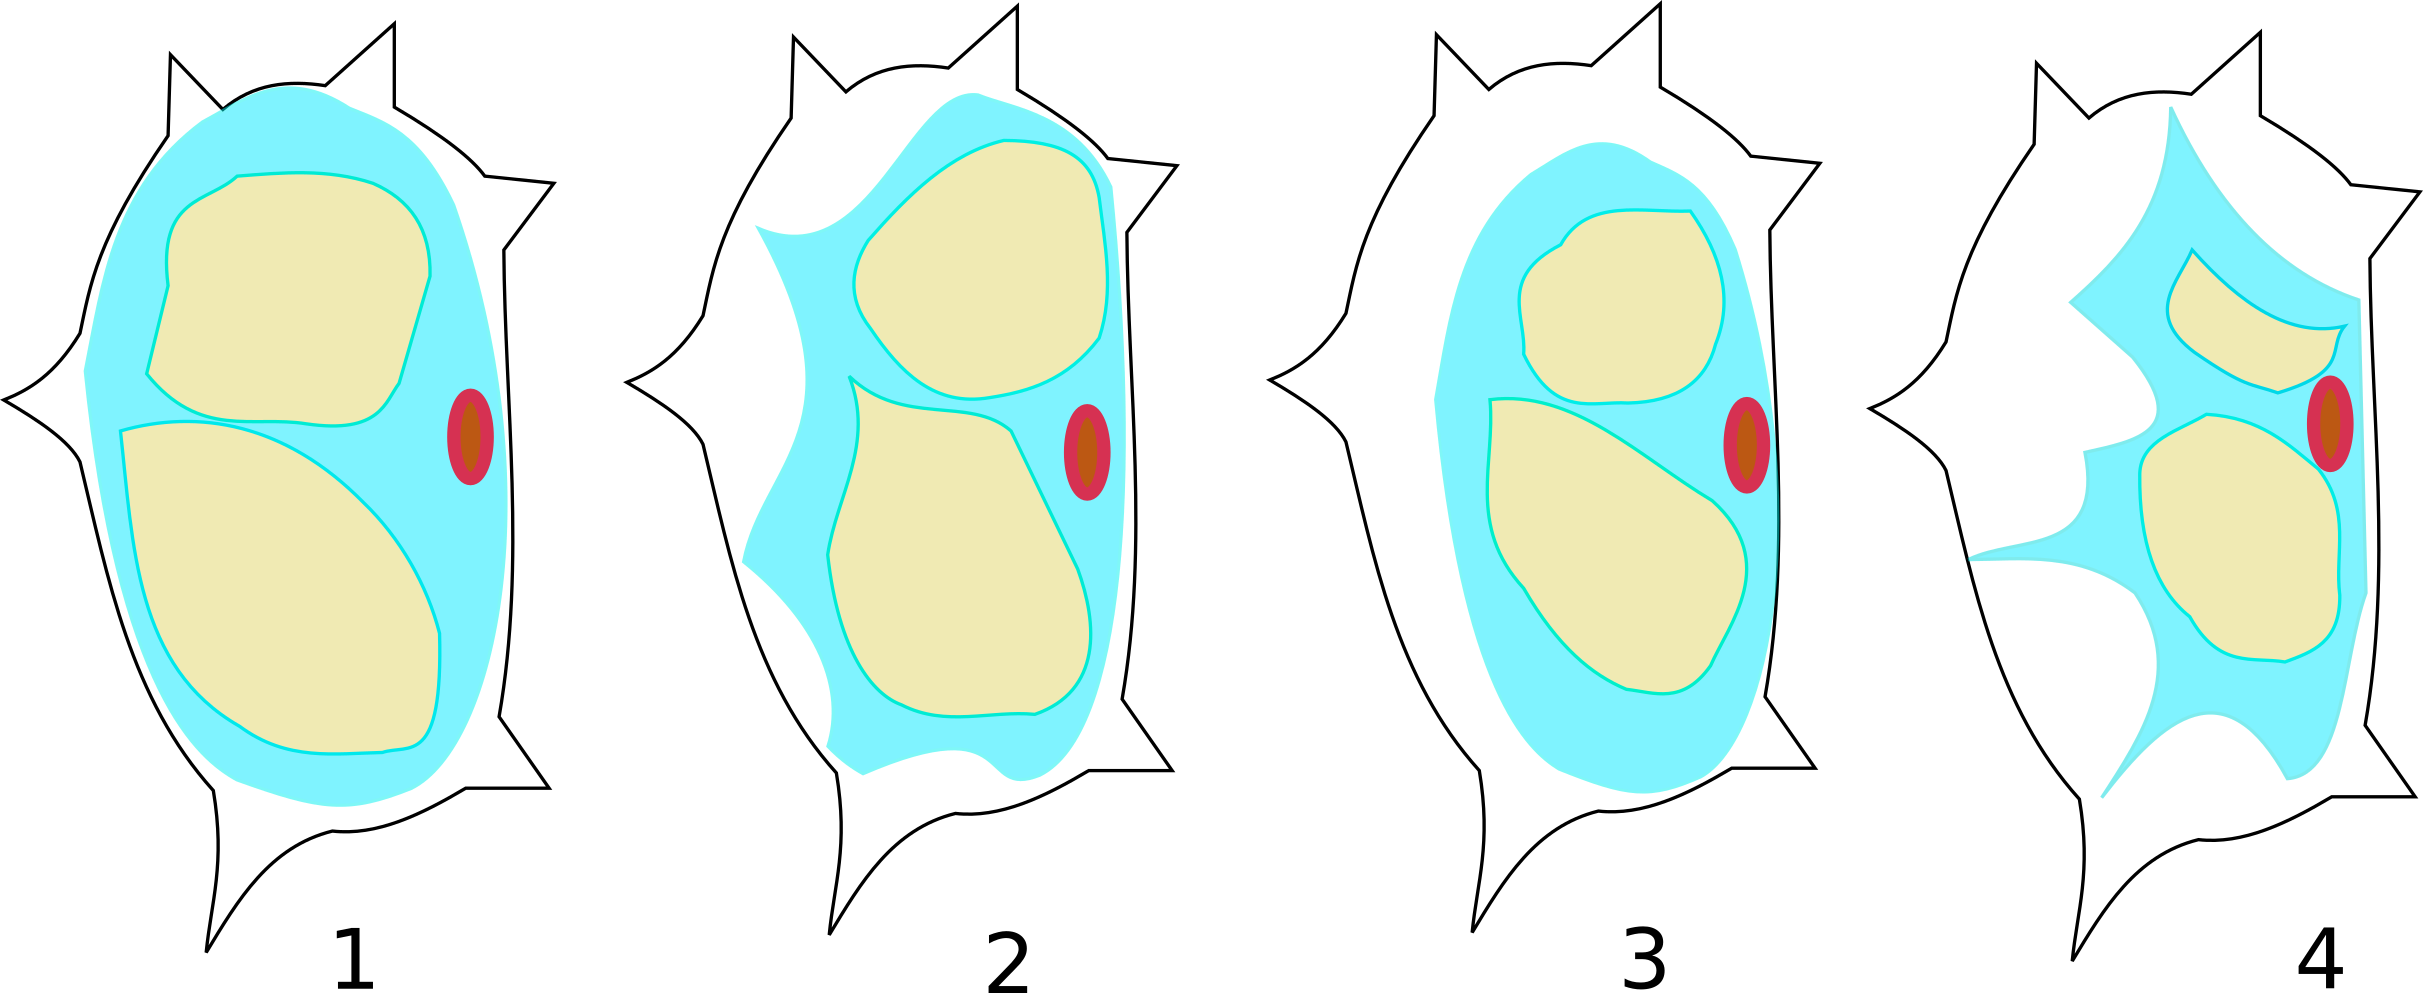
\includegraphics[width=0.5\linewidth]{pictures/plasmolis}
%\caption{Различные типы плазмолиза}
%\label{plasmolis_types}
%\end{figure}
%%%%%%%%%%%%%%%%%%%%%%%%%%%%%%%%%%%%%%%%%%%%%%%%%%%%%%%%%%%%%%%%%%%%%%%%%%%%%%%%%%%%%%%%%%%%%%%%%%%%%%%%%%%

%\paragraph*{}При определенных условиях, плазмолиз может быть \hyperlink{reversable_plasmolisys}{обратимым}. Явление обратное плазмолизу носит название \textit{деплазмолиз}.
%\paragraph{}Катионы и анионы солей оказывают специфическое и многообразное действие на цитоплазму. Одним из заметных внешних проявлений этого действия является изменение степени набухания и вязкости цитоплазмы. Чем выше вязкость цитоплазмы, тем медленнее наступает плазмолиз. Показателем, характеризующим особенности ответной реакции цитоплазмы на воздействие отдельных солей, служит время плазмолиза.

%\paragraph{}Одной из характеристик плазмолиза является время, необходимое для его начала. 

%\paragraph{}\efbox[margin=10pt,backgroundcolor=yellow]{
%	\begin{minipage}{0.95\textwidth}
%\textbf{Время плазмолиза} – это время, прошедшее от момента погружения ткани в гипертонический раствор соли, до наступления выпуклого плазмолиза (примерно у половины клеток в поле зрения микроскопа).
%	\end{minipage}
%	}

%\paragraph*{}Время наступления плазмолиза может зависеть от вязкости цитоплазмы. Чем выше вязкость цитоплазмы, тем медленнее наступает плазмолиз. В свою очередь на вязкость и степень набухания цитоплазмы оказывают влияние различные катионы, в первую очередь ионы K$^+$ и Ca$^{2+}$.


%\paragraph*{}При действии на клетку \hyperlink{hypertonik_liquid}{гипертонических} растворов солей, проникающих через плазмолемму, но не проходящих через тонопласт возникает \textit{колпачковый плазмолиз}, который проявляется  в образовании колпачков из набухшей цитоплазмы на концах плазмолизированного тонопласта.

%\paragraph*{}Соли, вызывающие колпачковый плазмолиз вызывают, кроме того, набухание цитоплазмы, денатурацию белков и увеличение светорассеяния.

\begin{footnotesize}

\paragraph*{}\textbf{Цель работы}: изучить, реакцию клетки на нарушение баланса катионов. Провести наблюдения плазмолиза различного типа

\paragraph*{}\textbf{Оборудование}: Луковица с пигментированными чешуями. Микроскопы, предметные и покровные стекла, бритвы, секундомер;

\paragraph*{}\textbf{Реактивы}: растворы солей: 0,7 \gls{mol} Ca(NO${_3}$)$_2$, 1 \gls{mol} KNO$_3$, 1 \gls{mol} KCNS;

\end{footnotesize}


\subsection*{Ход работы}

\paragraph*{}С выпуклой поверхности пигментированной чешуи лука срежьте участок эпидермиса и поместите его на предметное стекло в каплю раствора нитрата кальция. 

\paragraph*{}Накройте, подготовленный таким образом препарат кожицы лука, покровным стеклом и рассмотрите его под микроскопом, следя за сменой форм плазмолиза. 

\paragraph*{}С помощью секундомера определите время начала плазмолиза клеток.

\paragraph*{}Определите время плазмолиза для клеток эпидермиса, помещённых в раствор нитрата калия.

\paragraph*{}На примере препарата, помещённого в растворе родонида калия (KCNS) пронаблюдайте за наступлением колпачкового плазмолиза. 

\paragraph*{}Зарисуйте в альбом клетки, находящиеся на разных стадиях плазмолиза.

\paragraph*{}\textbf{Сделайте выводы}, в которых обоснуйте, каким образом плазмолиз доказывает тот факт, что цитоплазматическая мембрана является полупроницаемой.

\subsection*{Вопросы для самоконтроля}

	\begin{itemize}
		\item Дайте определение понятию \hypertarget{gomiostatsis_question}{гомеостаз}.
		\item Что такое осмотическое давление, в каких единицах оно измеряется. Что такое \hypertarget{hypertonik_liquid}{гипертонический}, гипотонический и изотонический растворы \cite{chem_kuzmenko_eremin}?
		\item От каких факторов зависит величина осмотического давления?
		\item Что такое тургорное давление?
		\item Наблюдаются ли различия в характере плазмолиза вызванного разными солями? Чем это можно объяснить?
		\item В растворах каких веществ будет наблюдаться \hypertarget{reversable_plasmolisys}{обратимый плазмолиз}? Почему?
		\item Способны ли плазмолизироваться мертвые клетки? Почему?
		\item Какова физическая природа процессов диффузии и осмоса?
		\item Каким образом ионы и вода проходят через цитоплазматическую мембрану клетки. В чем различия между активным и пассивным транспортом?
	\end{itemize}
